\subsection{Explicación detallada del algoritmo}

Como ya mencionamos en el ejercicio 2 este problema no parece poder ser resuelto en tiempo polinomial, para poder acercarnos a una solución en tiempos razonables sacrificaremos la seguridad de conseguir siempre la opción óptima a cambio de mejorar la complejidad temporal. Esto se hará a partir de la implementación de una heuristica golosa, un programa que a partir de ciertas suposiciones, no necesariamente validas siempre pero muchas veces útiles, nos permitirá tomar desiciones rapidamente. Será golosa porque tomará desiciones buscando mejorar su estado actual sin pensar en la solución optima final, o sea, sin pensar a largo plazo.

Hicimos dos versiones distintas. La primer versión consiste en mapear los nodos de mayor grado entre si hasta agotar todos los del grafo mas chico. Esto puede funcionar en algunos grafos pero claramente no siempre será la mejor opción.

\begin{algorithm}[H]
  \begin{algorithmic}[1]
  \caption{Pseudocódigo de la primer heurística golosa}
  \label{algo:4-1}
    \Procedure{goloso1}{\texttt{Grafo} $g1$, \texttt{Grafo} $g2$, \texttt{set<int>} $vertices1$, \texttt{set<int>} $vertices2$} $\to$ \texttt{MCS}
      \State $ordenar\_por\_grado(vertices1, g1)$ 
        \Comment $O(n_1^2)$ 
      \State $ordenar\_por\_grado(vertices2, g2)$ 
        \Comment $O(n_2^2)$ 
      \State \texttt{MCS} $solucion$ 
        \Comment $O(1)$ 

	  \For { \texttt{int} $i = 0$, $i < vertices1.tamanio()$, $i++$ }
	  \State  $solucion.isomorfismo.insertar\_atras(<vertices1[i],vertices2[i]>)$
      \Comment $n_1$ veces $O(1)$
    	  \EndFor

	  \State \texttt{int} $aristas$
	  \State $ aristas = contar\_aristas\_isomorfismo(g1,g2,u,v, solucion.isomorfismo)$
      \Comment $O(n_1^2)$
	  \State $solucion.aristas = aristas$
	  \Comment $O(1)$
      \State \Return $solucion$
      \EndProcedure
	\end{algorithmic}
\end{algorithm}

Como se puede observar en el pseudo-código, el programa inicia ordenando por grado los vértices con $ordenar_por_grado()$ ayudandose con las matrices de adyacencia de $g_1$ y $g_2$. Luego crea el isomorfismo escogiendo mapear el nodo de mayor grado de $g_1$ con el de $g_2$, luego el segundo y asi sucesivamente hasta que se agoten. Una vez hecho esto se calculan las aristas del isomorfismo con $contar_aristas_isomorfismo()$, verificando que aristas se comparten en ambos grafos. (Para mas detalles sobre las funciones nombradas recurrir al apéndice.)

La segunda heurística tiene una mayor complejidad temporal pero da soluciones de calidad superior, esto será expuesto en sección de experimentación. El algoritmo inicia haciendo un mapeo entre el nodo de mayor grado de $G_1$ y $G_2$ luego expande este isomorfismo buscando en cada iteración agregar el mapeo de nodos que maximice la cantidad de aristas (del isomorfismo). Si hay empates se queda con la primer opción.

El pseudocódigo es el siguiente

\begin{algorithm}[H]
  \begin{algorithmic}[1]
  \caption{Pseudocódigo de la heurística golosa}
  \label{algo:4-1}
    \Procedure{goloso}{\texttt{Grafo} $g1$, \texttt{Grafo} $g2$, \texttt{vector<int>} $vertices1$, \texttt{vector<int>} $vertices2$} $\to$ \texttt{MCS}
      \State \texttt{MCS} $solucion$ 
        \Comment $O(1)$ 
      \State $solucion.aristas = 0$ 
      \State \texttt{int} $vertice1 = mayor\_adj(vertices1,g1)$ 
      \Comment $O(n_1)$ 
      \State \texttt{int} $vertice2 = mayor\_adj(vertices2,g2)$ 
      \Comment $O(n_2)$ 
      \State $solucion.isomorfismo.insertar\_atras(<vertice1,vertice2>)$
      \Comment $O(1)$
      \State $vertices1.borrar(vertice1)$ 
      \Comment $O(\log(n_1))$ 
      \State $vertices2.borrar(vertice2)$ 
      \Comment $O(\log(n_2))$
      \While {$ vertices1.tamanio() \neq 0 $}
	  \State \texttt{par<int,int>}  $par\_mayor\_deg = <vertices1.primero(),vertices2.primero()>$ 
    \Comment $n_1$ veces $O(1)$
	  \For { $u \in vertices1$ }
	  \For { $v \in vertices2$ }
	  \State \texttt{int} $aristas$
    \Comment $n_1^2n_2$ veces $O(1)$
	  \State $ aristas = contar\_aristas\_isomorfismo(g1,g2,u,v, solucion.isomorfismo)$
    \Comment $n_1^2n_2$ veces $O(n_1^2)$
      \If { $aristas > solucion.aristas$}
      \Comment $n_1^2n_2$ veces $O(1)$
      \State $solucion.aristas = aristas$
      \Comment $n_1^2n_2$ veces $O(1)$
      \State $par\_mayor\_deg = <u,v>$
      \Comment $n_1^2n_2$ veces $O(1)$
      \EndIf
	  \EndFor
	  \EndFor	 
	  \State  $solucion.isomorfismo.insertar\_atras(par\_mayor\_deg)$
      \Comment $n_1$ veces $O(1)$
	  \State $ vertices1.borrar(par\_mayor\_deg.primero)$
      \Comment $n_1$ veces $O(\log(n_1))$
	  \State $ vertices1.borrar(par\_mayor\_deg.segundo)$
      \Comment $n_1$ veces $O(\log(n_2))$
	  \EndWhile      
        \State \Return $solucion$
      \EndProcedure
	\end{algorithmic}
\end{algorithm}



\subsection{Complejidad temporal de peor caso}

El primer algoritmo tiene complejidad $O(n_2^2 + n_1^2)$ lo cual es acotable superiormente por $O(n_2^2)$ ya que $n_2$ siempre es mayor que $n_1$, es la precondición del programa. 

En la segunda heuristica la complejidad es precisamente $O(n_1^4 n_2)$. Esto resulta de los 3 ciclos anidados que hay mas una operación de costo cuadratico respecto de $n_1$. Si sumamos todo lo que se detalló en el pseudocódigo se puede ver que queda $O(n_1 + n_2 + \log(n_1) + \log(n_2) + n_1^2.n_2 + n_1^2.n_2.n_1^2 + n_1.\log(n_1) + n_1.\log(n_2)) = O(n_1^4 n_2)$

\subsection{Instancias no óptimas}

La primer heuristica tiene varios casos donde fallará rotundamente. Un ejemplo puede ser el caso en que $G_1$ es el grafo completo $G_n$ y $G_2$ la unión de $n$ grafos estrella $S_n$. En ese caso, por el funcionamiento de nuestro algoritmo, se mapeará a cada nodo del grafo completo con el centro de cada una de las $n$ estrellas, ya que los centros de las estrellas son los nodos de mayor grado, esto formará un isomorfismo sin aristas, ya que en $G_2$ todos los nodos escogidos son disconexos entre si. Esta solución será mucho peor que la óptima que se dá al tomar el centro de una estrella y $n-1$ nodos conexos a este y mapearlos a los del grafo completo, la solución óptima tiene $n$ aristas.


Un ejemplo donde la segunda heuristica golosa puede ser tan mala como uno quiera es cuando en su entrada recibe al grafo completo $G_n$ y a un grafo que resulta de la unión de $G_n$ con $S_n$, el cual es ilustrado mas abajo. 

\begin{tikzpicture}[shorten >=1pt,auto,node distance=1.9cm,
                    semithick]
  \tikzstyle{every state}=[fill=red,draw=none,text=white]

	\node[state]	(0)		 		  {$2$};
	\node[state]	(1) [right of=0]  {$4$};
	\node[state]	(2) [below of=0]  {$3$};
	\node[state]	(3) [left of=0] 	  {$0$};
	\node[state]	(4) [above of=0]	  {$1$};
	\node[state]	(5) [right of=1]	  {$5$};
	\node[state]	(6) [above of=5]  {$6$};
	\node[state]	(7) [right of=6]  {$7$};
	\node[state]	(8) [right of=5]  {$8$};
	\node[state, fill=blue]	(9) [right of=8]	  {$0$};
	\node[state, fill=blue]	(10) [above of=9]  {$1$};
	\node[state, fill=blue]	(11) [right of=9]  {$2$};
	\node[state, fill=blue]	(12) [right of=10]  {$3$};


	\path	
		(0) edge[]				node {} (1)
         	edge[]				node {} (2)
         	edge[]				node {} (4)
         	edge[]				node {} (3)
		(1) edge[]				node {} (5)
		(5) edge[]				node {} (6)
		    edge[]				node {} (7)
		    edge[]				node {} (8)
		(6) edge[]				node {} (7)
		    edge[]				node {} (8)
		(7) edge[]				node {} (8)
		(9) edge[]				node {} (10)
		    edge[]				node {} (11)
		    edge[]				node {} (12)
		(10) edge[]				node {} (11)
		    edge[]				node {} (12)
		(11) edge[]				node {} (12);

\end{tikzpicture}

Si recordamos como funciona la segunda heuristica golosa será entendible que arrancará mapeando el centro de la estrella con algun nodo del grafo completo. Luego seguirá con un nodo que maximice la cantidad de aristas del isomorfismo, el primero que encontrará que cumpla esto será  el nodo 0, seguirá de esta manera mapeando los extremos de la estrella con los nodos del grafo completo. En vez de elegir la opción óptima, mapear el grafo completo con el grafo completo contenido en $G_1$.

Para estos casos la salida de la heuristica, $H(n)$, siempre va a devolver un isomorfismo con $n$ aristas, ya que mapeara los nodos de la estrella con los del grafo completo. En vez de esto la solución óptima, $Opt(n)$, sería $G_n$, o sea tendría $\frac{n.(n-1)}{2}$ aristas, por lo cual este no es un algoritmo aproximado, para $n$ suficientemente grande no existe ningun número real positivo, $\rho$, que acote inferiormente a $\frac{H(n)}{Opt(n)} = \frac{n}{n.(n-1)/2} = \frac{2}{n-1}$.

\subsection{Performance del algoritmo}
\subsection{Experimentación}

En esta parte del informe nos dedicaremos principalmente a corroborar empíricamente ciertas hipótesis sobre nuestra segunda heurística golosa.

Primero intentamos ver que la complejidad del peor caso, $\O(n_1^4.n_2)$ sea una cota superior correcta. Esto es corroborado en el siguiente gráfico.

\begin{figure}[H]
 \centering
	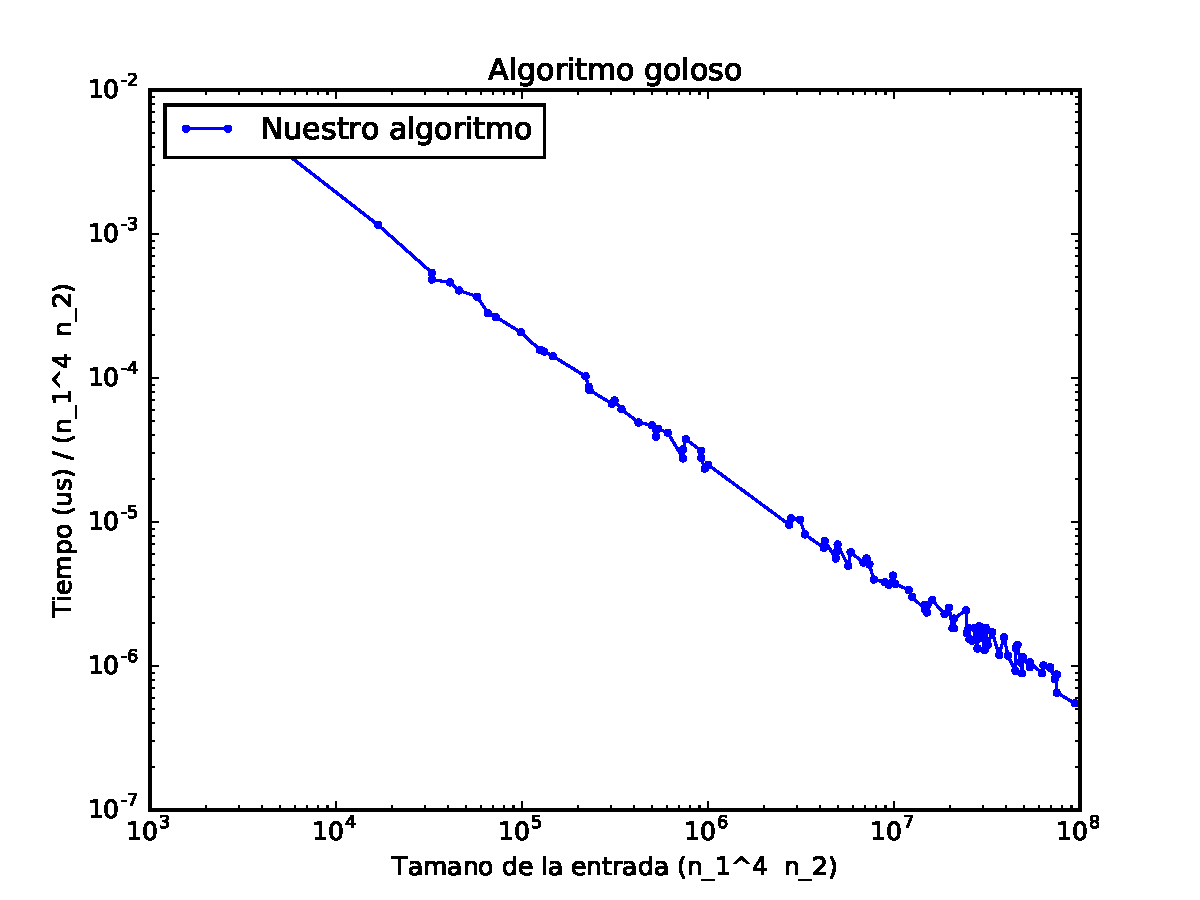
\includegraphics[width=0.9\textwidth]{graficos/problema_4/tiempos_1.pdf}
	\caption{}
	\label{fig:problema4-1}
\end{figure}

Se puede observar como, para instancias cada vez mas grandes, el tiempo en relación a la cota esperada decrece tendiendo a cero, de esto se puede deducir que nuestra cota no es la mas ajustada posible, o sea no serviría al mismo tiempo como cota inferior.

Como se puede observar, la complejidad que calculamos previamente depende de dos variables, $n_1$ y $n_2$, los siguientes gráficos analizan por separado que pasa cuando se varía cada uno de estos valores y se intenta corroborar que la complejidad es correcta.

\begin{figure}[H]
 \centering
	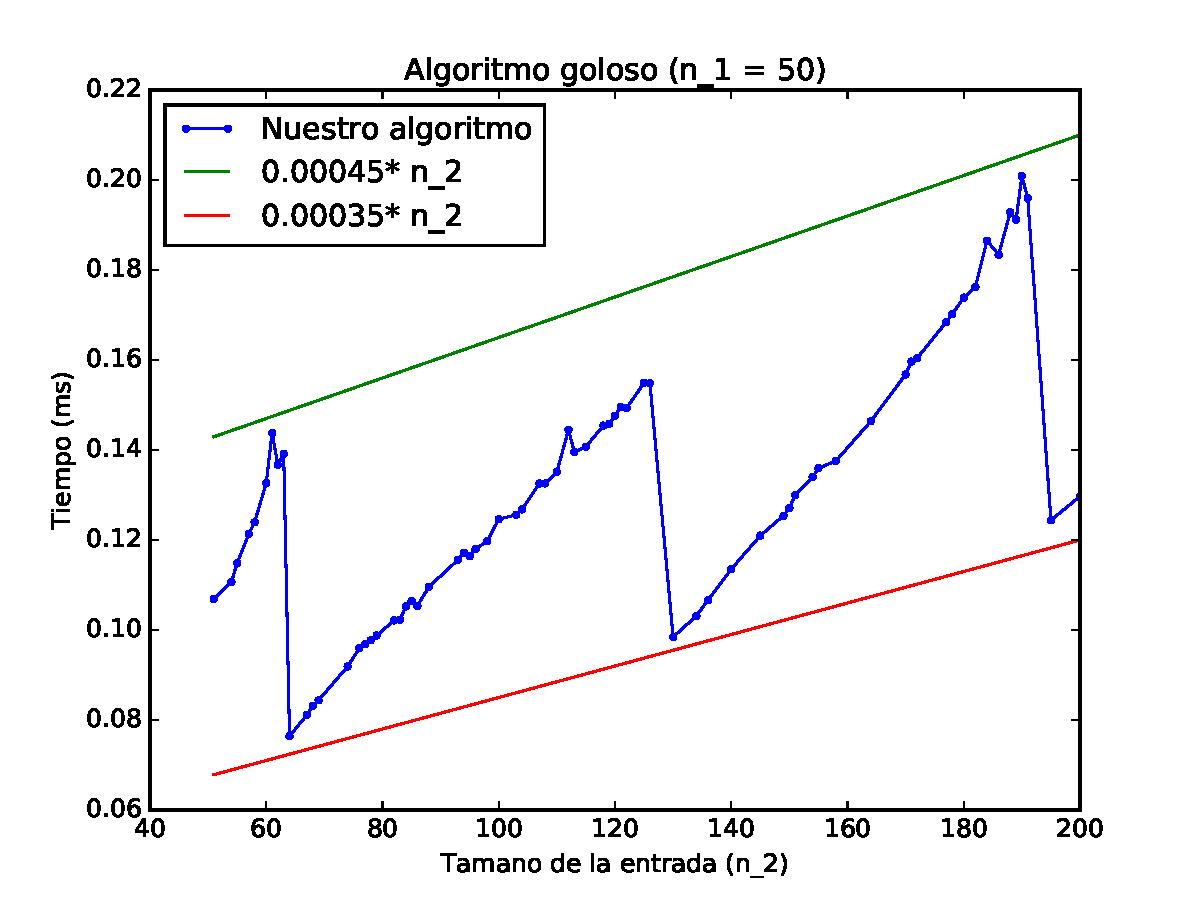
\includegraphics[width=0.9\textwidth]{graficos/problema_4/tiempos_2.pdf}
	\caption{}
	\label{fig:problema4-2}
\end{figure}

Este gráfico tiene dos particularidades que vale la pena comentar. Primero que púdimos ajustar el problema inferior y superiormente para esta variable. Segundo que hay picos, esto se debe a la manera en que maneja c++ a los vectores, estos se copian y aumentan de tamaño al pasar un tamaño multiplo de 64 elementos.

\begin{figure}[H]
 \centering
	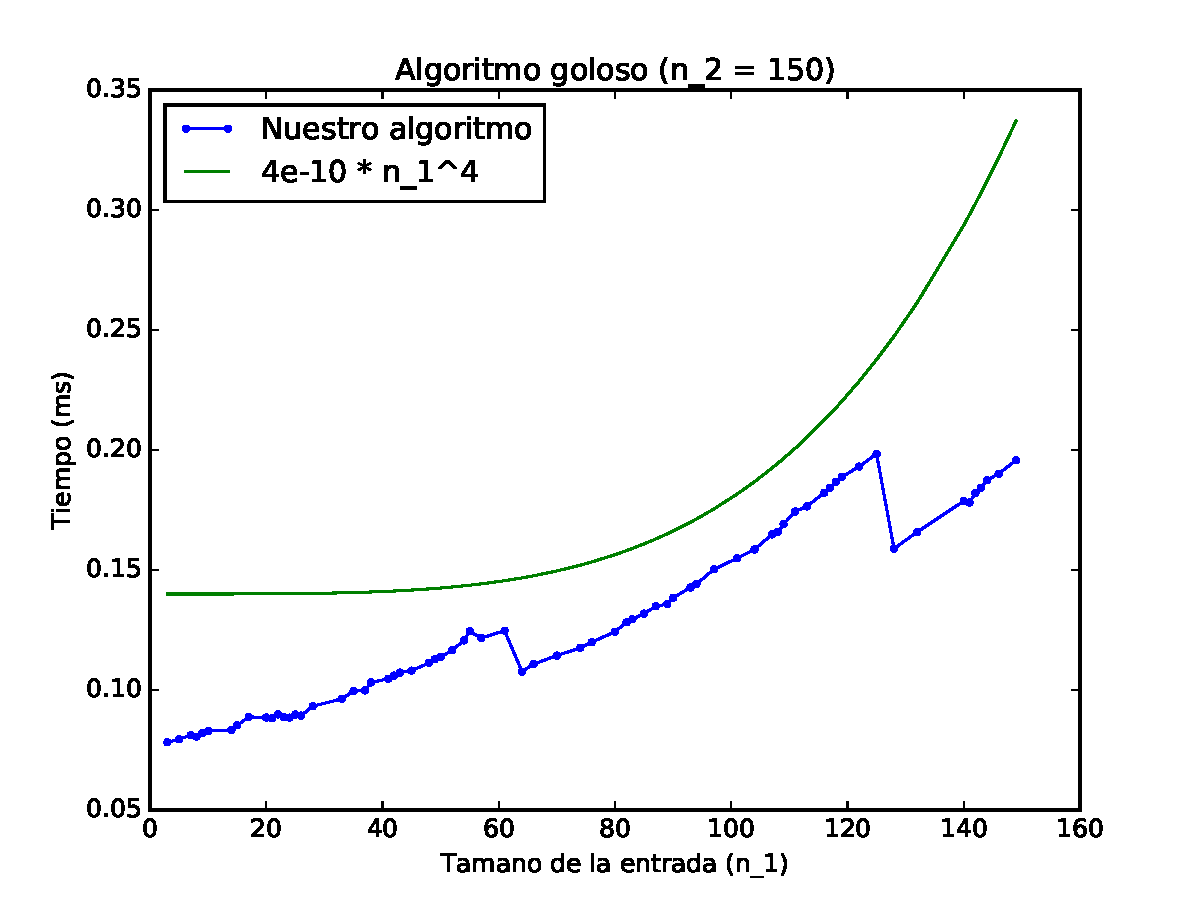
\includegraphics[width=0.9\textwidth]{graficos/problema_4/tiempos_3.pdf}
	\caption{}
	\label{fig:problema4-3}
\end{figure}

En este gráfico se ve como acotamos superiormente las instancias generadas con la complejidad que habiamos calculado, variando solo $n_1$.

La siguiente fígura expone la cantidad de aristas que tenian los isomorfismos calculados por nuestras dos heurísticas golosas, la mala (la primera) y la segunda, la que escogimos como nuestro algoritmo predilecto.

\begin{figure}[H]
 \centering
	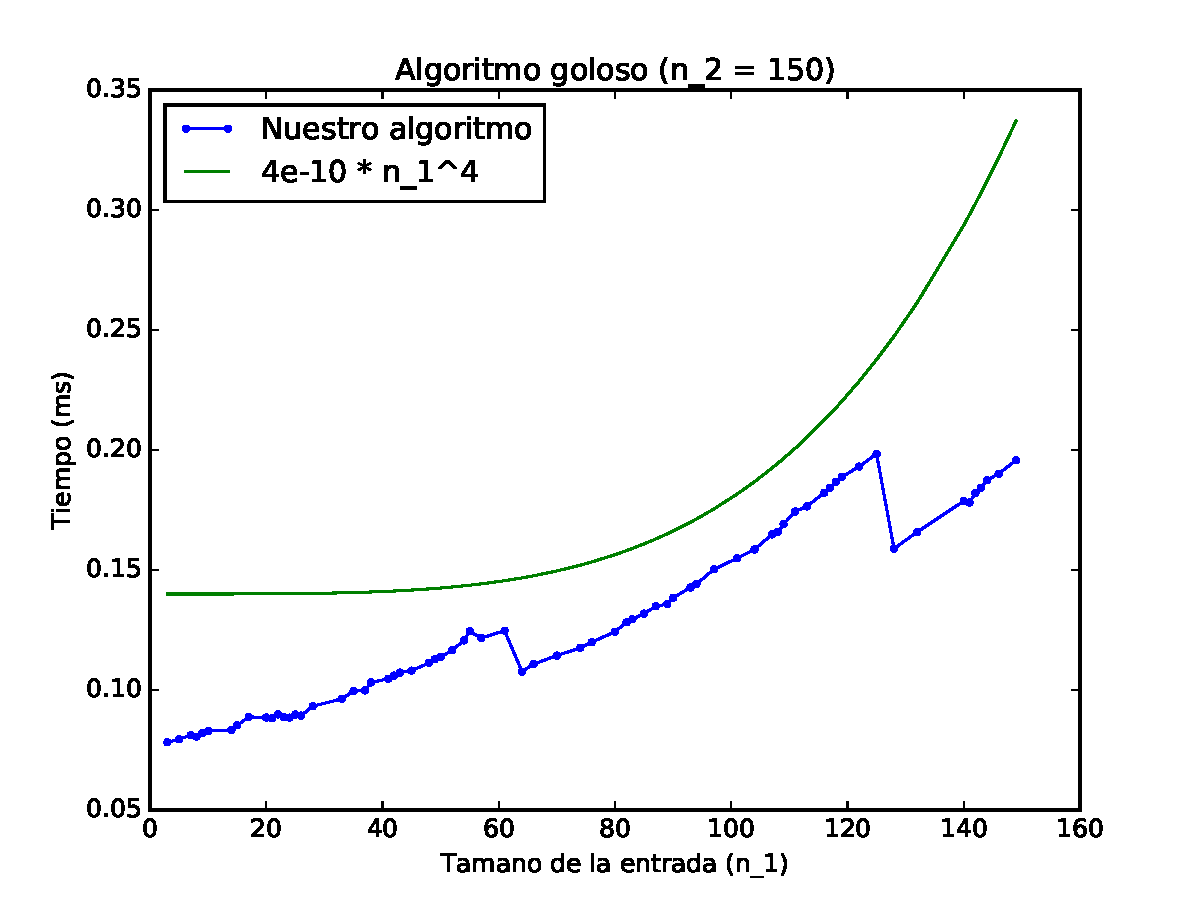
\includegraphics[width=0.9\textwidth]{graficos/problema_4/calidad.pdf}
	\caption{}
	\label{fig:problema4-4}
\end{figure}

Se puede ver como nuestro algoritmo siempre es en promedio superior en todos los casos. Aunque la ventaja no es  inmensa tampoco, lo cual deja a criterio de la aplicación deseada si es preferible usar una u otra, ya que si recordamos lo dicho antes, la complejidad del Goloso Malo es bastante mejor, $O(n_2^2)$.

\subsection{Método de experimentación}

